\documentclass[11pt]{article}

\usepackage{geometry}
\geometry{a4paper, portrait, margin=3cm}

\usepackage{todonotes}
%TC:macro \todo [ignore]

\usepackage{helvet}
\renewcommand{\familydefault}{\sfdefault}

\usepackage[utf8]{inputenc}
\usepackage{amsmath}
\usepackage{setspace}
\usepackage{indentfirst}
\usepackage{siunitx}
\usepackage{amssymb}
\usepackage{parskip}
\usepackage{lineno}
\usepackage{graphicx}
\usepackage[labelfont=bf]{caption}
\usepackage{float}
\usepackage[authoryear]{natbib}
\usepackage[T1]{fontenc}

%opening

\begin{document}

	\begin{titlepage}
		
		
\includegraphics[width = 5cm]{../results/images/imperial.pdf}
		
		\begin{center}
			
		\vspace*{2cm}
		\LARGE
		CMEE MiniProject:
		
		\vspace*{3cm}
		\Huge
		\textbf{Comparison between Mechanistic Model and Phenomenological Model fitting on growth rate data}\\
		
		\vspace{5cm}
		\Large
		
		\textbf{Student:} Hongye Wang \textit{(hw2419@ic.ac.uk)}\\
		\vspace*{1cm}
		\textbf{Affiliation:} Department of Life Sciences. Imperial College London\\
		\vspace*{1cm}
		\textbf{Word Count:} 3603
		
		\vspace{2cm}
		
		\end{center}

	\end{titlepage}
	
\clearpage
\tableofcontents
	
	
\linenumbers
\doublespacing
\section{Abstract}
In order to estimate bacterial growth kinetics, many sigmoidal functions were compared to fit the growth curves. In this report, the tested models are Classical mechanistic model, Gompertz model, Baranyi model, Buchanan model and Cubic model. The aim of my work is to find the best fitted one. They were fitted by the methods of NLLS fitting. The outcomes were compared and analyzed under the condition of $AIC$, $AICc$, $\Delta$$AIC$, $\Delta$$AICc$ and Akaike Weight. Eventually, Classical mechanistic model provided the best fit result among all models. 



\section{Introduction}
The use of primary mathematical models with curve fitting software is more and more welcomed in the microbiology field. Food microbiologists use the way of predictive modeling to analyze the bacterial growth data and estimate the microbial safety or shelf life of products\citep{zwietering1990modeling}.
The prediction model mainly expresses the functional relationship between the time and the population of microorganisms, i.e. the response of the microorganisms, and the equation is expressed by a series of specific parameters. The parameters are divided into two types: direct response parameters and indirect response parameters. In recent years, researchers have proposed many mathematical equations describing the dynamic growth of microorganisms, including Gompertz equation, Logistic equation, Baranyi equation and Buchanan equation, which will be described in detail below.

The aim of my work is to find the best fitted model which can be used to estimate bacteria growth.

    \subsection{Bacterial growth curve}
    The growth curve is represented by the dotted line on the graph of the growth phenomenon. Under the proper growth conditions, the bacterial population increased in the schizont way and show an exponential explosion\citep{eagon1962pseudomonas}. The growth curve drawn with the logarithm of the number of bacterial cells as the ordinate and the growth time as the abscissa, also called a sigmoid curve, which can be divided into four parts, reflecting the four main stages of bacterial growth\citep{baty2004estimating}: lag phase, logarithmic phase, stationary phase and decline phase. 1. lag phase: generally, bacteria need a brief period to adapt the new environment. The curve in this period is flat and stable, because the bacteria reproduce very little, and the reproduction speed gradually increases from zero\citep{bertrand2019lag}. We use $N_0$ to represent the initial value of the bacterial population, and $t\textsubscript{lag}$ to represent the period of time when the proliferation rate changes from 0 to the maximum rate. 2. logarithmic phase: also called the exponential growth phase. After the preparation period of the lag phase, the bacteria grew extremely fast with a stable geometric progression, and therefore achieved the maximum growth rate($r\textsubscript{max}$), which showed a rapid rise in the growth curve and an exponential increase in the population of bacteria. In the end of logarithmic phase, the maximum population number($N\textsubscript{max}$) should be reached. 3. stationary phase: the growth curve in this period became to a horizontal line, which is call an asymptote($A$), but the bacterial population vigor changed greatly. Due to the adverse effects of nutrient consumption in the culture medium, toxic products (organic acids, H\textsubscript{2}O\textsubscript{2}, etc.) and the change of pH, the bacterial reproduction rate gradually decreased, and the relative number of bacterial deaths began to increase gradually\citep{bridges2001effect}. As a result, the number of bacterial proliferation and death finally balanced. 4. decline phase: with the development of the stable period, the bacteria multiply slowly and the number of dead bacteria increases significantly. The number of viable bacteria was inversely related to the culture time, and the growth curve began to fall\citep{novick1955growth}. However, in this article, we only consider the first three phases of the bacterial growth curve during the mode fitting process.
    
    \subsection{Models}
    1. Classical mechanistic model
    \begin{equation}
		N_{t} = \frac{N_0N_{max}e^{rt}}{N_{max} + N_0(e^{rt} - 1) }
		\end{equation}
		
    A classical mechanistic model is the logistic equation. Here $N_t$ is population size at time t, $N_0$ is initial population size, $r$ is maximum growth rate (AKA $r\textsubscript{max}$), and $N\textsubscript{max}$ is carrying capacity (commonly denoted by $K$ in the ecological literature).

    2. Gompertz model \citep{zwietering1990modeling}
    
    \begin{equation}
		N_{t} = Ae^{-e^{\frac{r_{max}e^{t_{lag}-t}}{A} + 1}}
		\end{equation}
		
	Gompertz model is one of the most widely used mathematical model, which has been modified now to model bacterial growth\citep{gibson1988predicting}. Here maximum growth rate ($r\textsubscript{max}$) is the tangent to the inflection point, $t\textsubscript{lag}$ is the x-axis intercept to this tangent (duration of the delay before the population starts growing exponentially) and $A$ is the asymptote ($A$ = $\ln$ (N\textrm{max}/N\textrm{0})), N\textsubscript{0} is initial cell culture (Population) density, N\textsubscript{max} is maximum population density.
	
	3. Baranyi model\citep{baranyi1993non}
	
	 \begin{equation}
		N_{t} = N_0 + r_{max}A_{t} - \ln (1 + \frac{e^{r_{max}A_{t}-1}}{e^{N_{max}-N_o}}
		\end{equation}
		
	Where:
	\begin{equation}
		A_{t} = t + \frac{1}{r_{max}}\cdot\ln (\frac{e^{-r_{max}t+h_0}}{1+h_0})
		\end{equation}
	
	Here h\textsubscript{0} represents the initial physiological state of the cells. The length of the lag phase is determined by the value of h\textsubscript{0} at inoculation and the post-inoculation environment. Thus the definition of lag is independent from the shape of the growth curve, and the effect of the previous environment is separated from the effects of the present environment. In this model, r\textsubscript{max} and h\textsubscript{0} can be related to obtain the t\textsubscript{lag}:	
	\begin{equation}
	    t_{lag} = \frac{\ln (1+\frac{1}{h_0})}{r_{max}}
	\end{equation}
	
	4. Buchanan model
	Buchanan model is a three-phase linear model, which use three line segments represent the three phases of bacterial growth\citep{buchanan1997simple}.
	
	\begin{align}
    Lag-phase: N_{t} &= N_0          &  t &<=t_{lag}\\
    Logarithmic-Phase: N_{t} &= N_0 + \mu(t-t_{lag})         &  t_{lag}&< t < t_{max}\\
    Stationary-Phase: N_{t} &= N_{max}   &  t&>=t_{max}        
    \end{align}

    where: N\textsubscript{t} is log of the population density at time t; N\textsubscript{0} is log of the initial population density; N\textsubscript{max} is log of the maximum population density supported by the environment; t is Elapsed time; t\textsubscript{lag} is the time when the lag phase ends; t\textsubscript{max} is the time when the maximum population density is reached; $\mu$ represents specific growth rate\citep{buchanan1990mathematical}.
    
    5. cubic polynomial model
    \begin{equation}
	    N_{t}= B_0 + B_1t + B_2t^2 + B_3t^3
	\end{equation}
	This is a phenomenological model, with the parameters $B_0$, $B_1$, $B_2$ and $B_3$ lacking any mechanistic interpretation. $t$ is the independent variable
	
\section{Methods}
    \subsection{Data Preparation}
    The first thing we need to do is to browse and reorganize the data we used for model fitting (Fig.1).
    \begin{figure}[H]
            \centering
			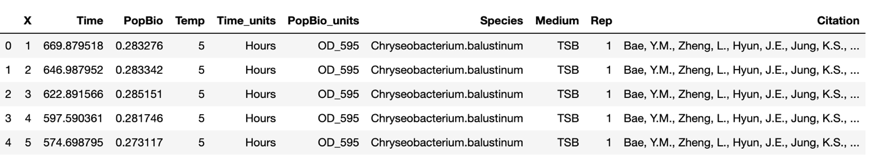
\includegraphics[width = \textwidth]{../results/images/Fig1.png}
            \caption{Initial database with the column headers}
            \label{fig1}
    \end{figure}
    
    I categorize the data by species, citation and rep, and create unique IDs for each group in the data frame, which is more convenient for building subsets when modeling fitting and plotting. Then, remove unusual data, such as those with a time of less than zero, or an empty set. After that, filter out the data subsets with less than 5 data points, because 5 is the minimum number of data points needed to fit the models. At last, log the data in the 'PopBio' column, store the results in a new column and rename them as 'log-popbio'. After preparation work, there are 295 available subsets grouped by ID, each group will be used to fit five models.
    
    \subsection{Find the starting value}
    It is important to finding appropriate starting value for each parameter in Non-linear Least Squares(NLLS) fitting method. Table.1 shows how many parameters each model has and what they are.
    \begin{table}[H] \centering
        \label{table1}
        \resizebox{\textwidth}{!}{%
        \begin{tabular}{c|c}
            \hline
            Model & Parameters \\
            \hline
            Classical mechanistic model & $N_0$, $N\textsubscript{max}$, $r\textsubscript{max}$\\
            Gompertz model & $A$, $t\textsubscript{lag}$, $r\textsubscript{max}$\\
            Baranyi model & $N_0$, $N\textsubscript{max}$, $r\textsubscript{max}$, $h_0$\\
            Buchanan model & $N_0$, $N\textsubscript{max}$, $t\textsubscript{lag}$,  $t\textsubscript{max}$, $\mu$\\
            cubic polynomial model & $B_0$, $B_2$, $B_3$, $B_4$\\
            \hline
        \end{tabular}}
        \caption{Five selected models and their parameters}
    \end{table}
    
    Since all the models have been re-parameterized to substitute the matical parameters with $A$, $t\textsubscript{lag}$ and $r\textsubscript{max}$(except the cubic) which made them can be calculated directly, now the models are easily to share the starting values in terms of same parameters. The method of finding starting value is as follows:
    
    $N_0$: the initial population size of each ID group.
    
    $N\textsubscript{max}$: the maximum population size of each ID group.
    
    $r\textsubscript{max}$: the steepest slope of the growth curve. Searching for the maximum slope is little more complicated. I sorted the points in the subset by time order, then draw a straight line every four points using Ordinary Least Squares(OLS) starting from the first point. Finally, comparing these line, the maximum slope is the value of $r\textsubscript{max}$(Fig.2).
    
    \begin{figure}[H]
            \centering
			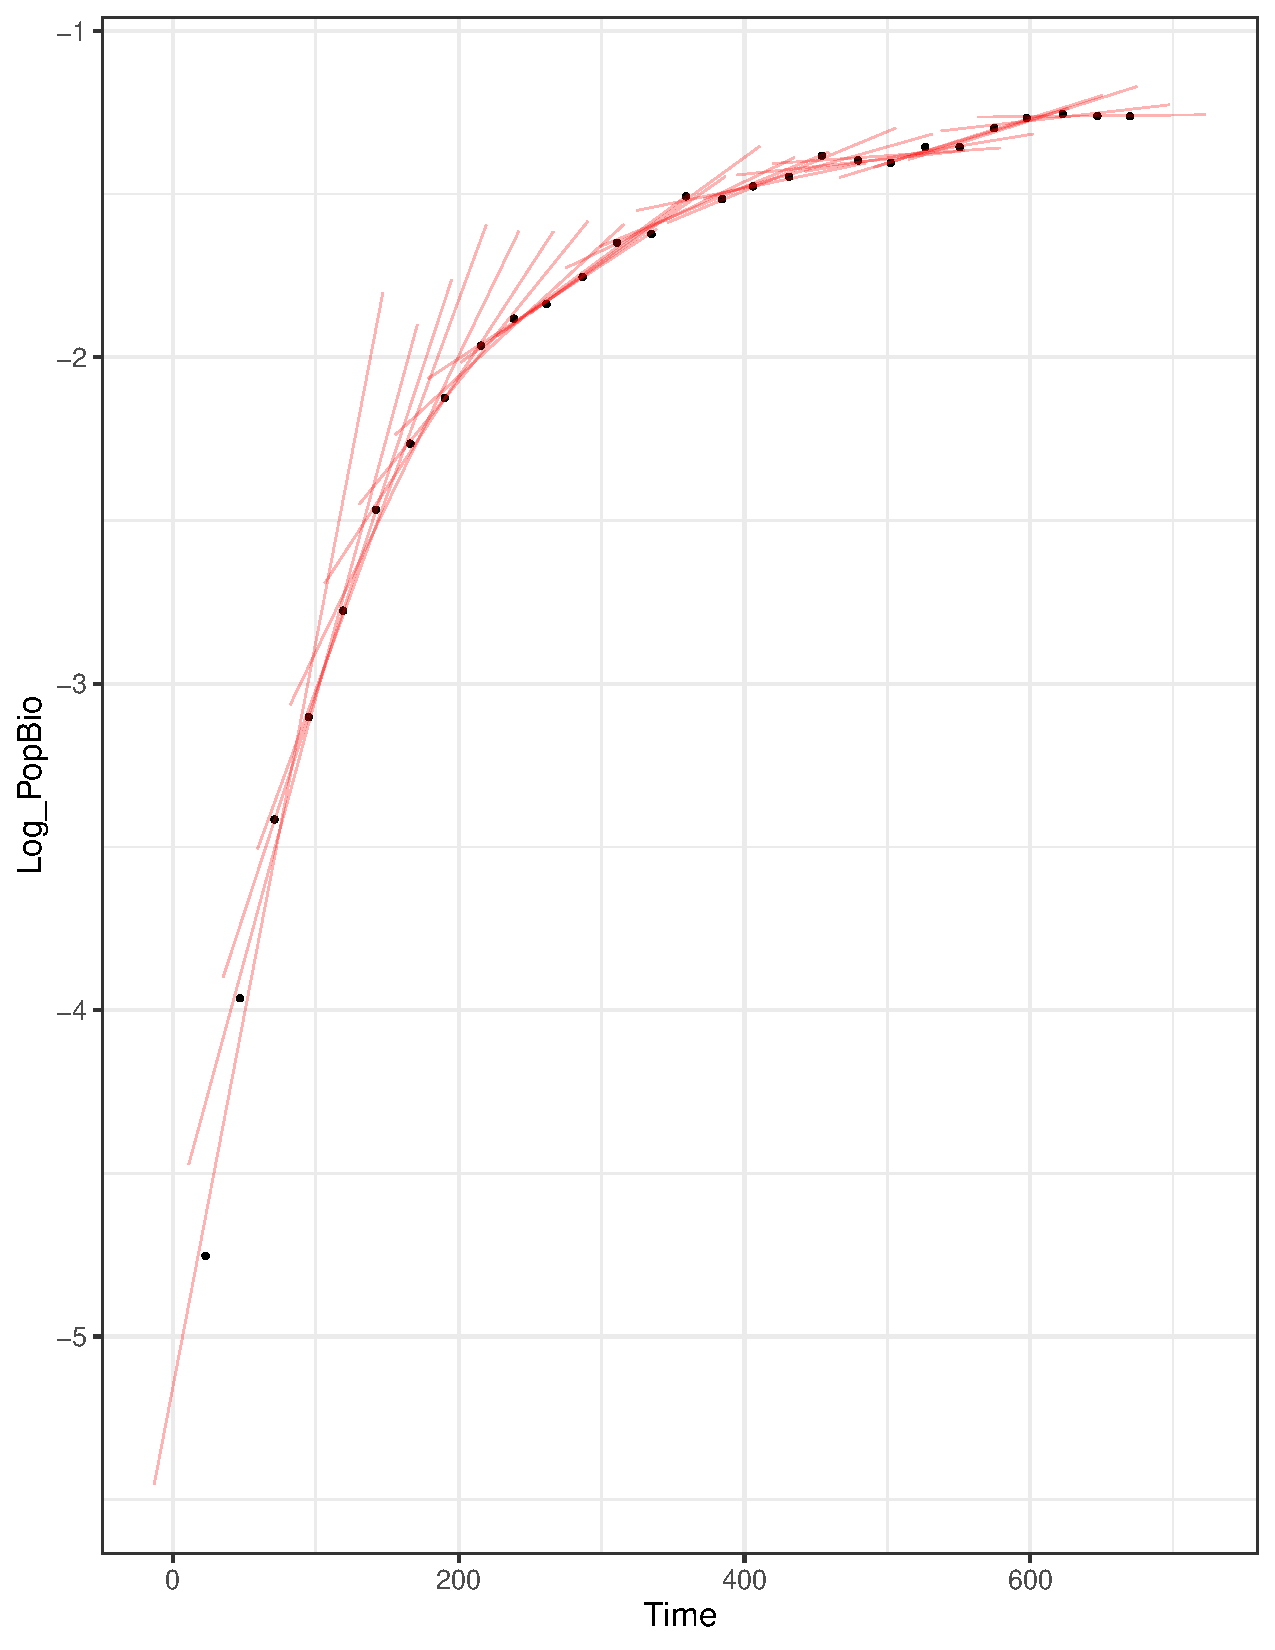
\includegraphics[width = \textwidth]{../results/images/find_rmax_sample1.pdf}
            \caption{Plotting rolling regression in a data subset (ID is 1) }
            \label{fig2}
    \end{figure}
    
    $\textsubscript{lag}$: The x-intercept created by the line with maximum slope.(Fig.3)
    
    \begin{figure}[H]
            \centering
			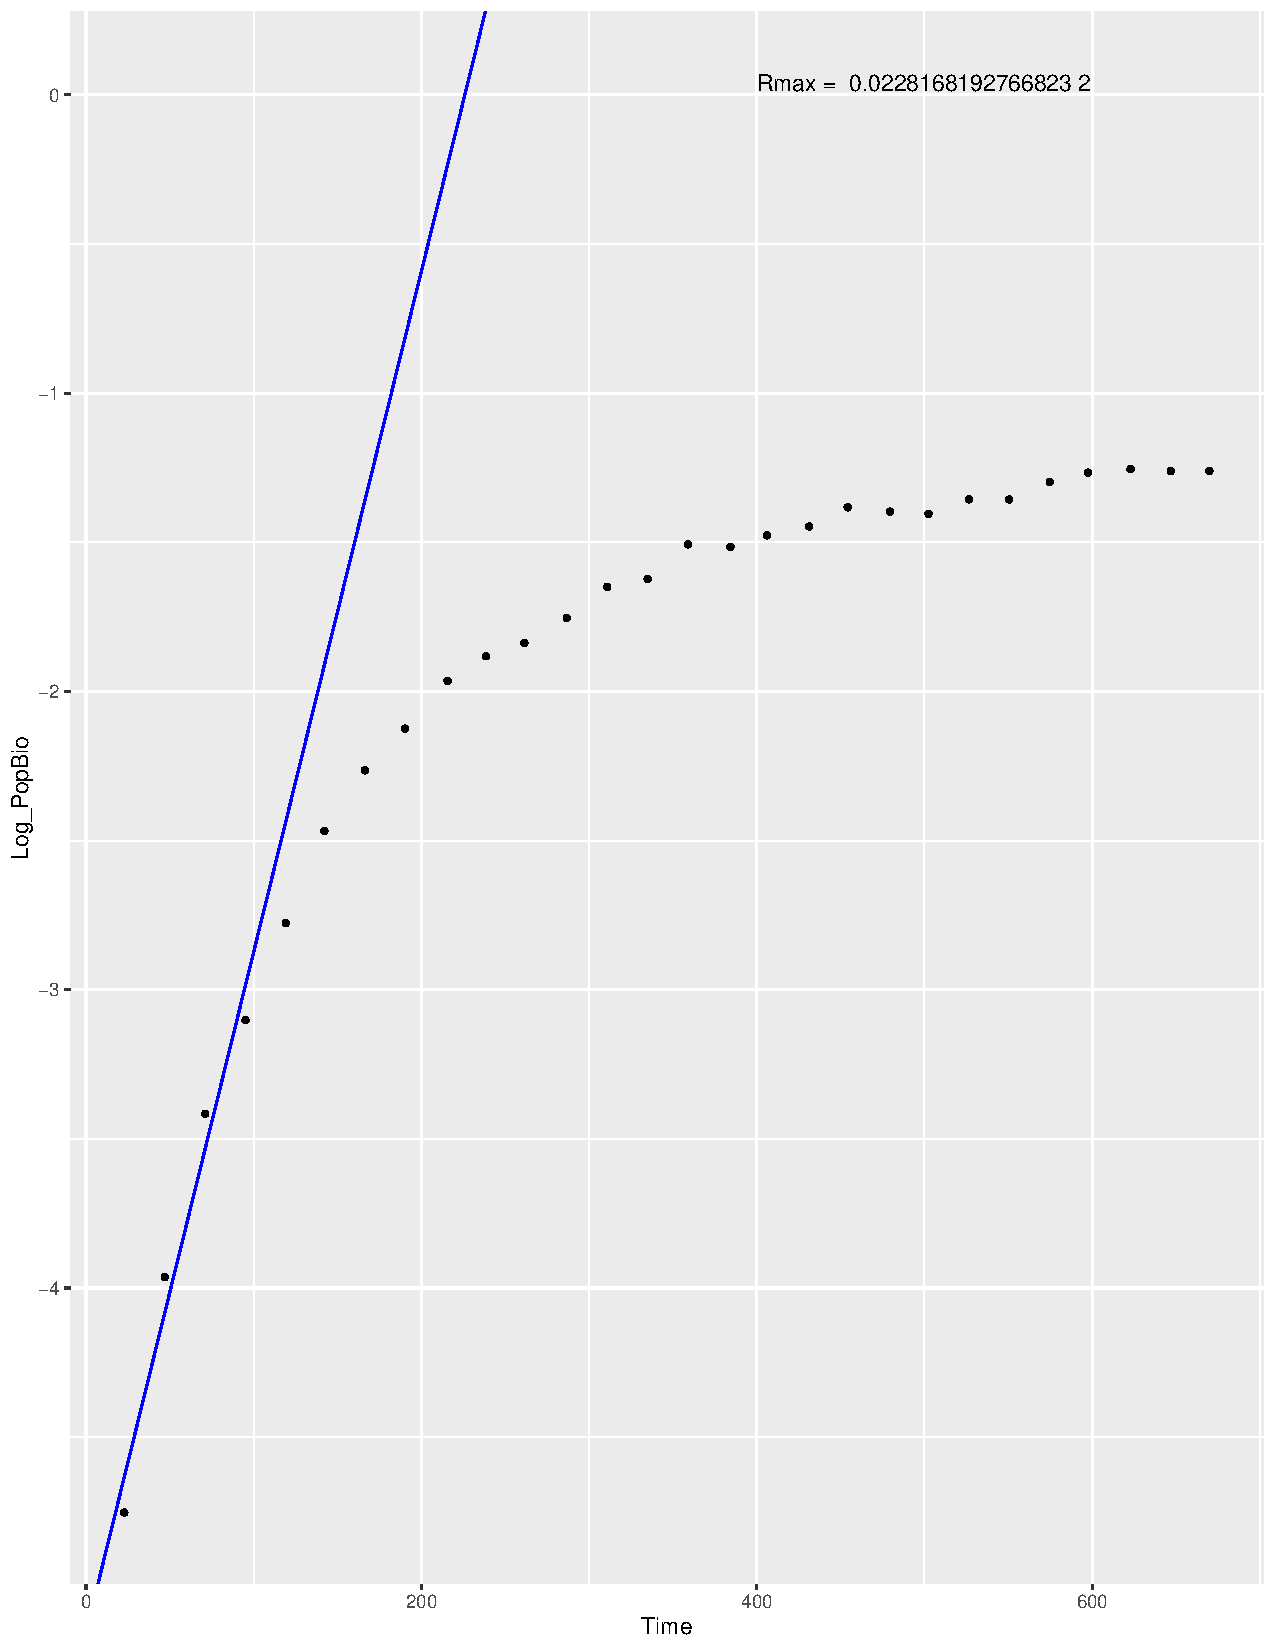
\includegraphics[width = \textwidth]{../results/images/Rmax_line_sample1.pdf}
            \caption{The line with the maximum slope and show the $R\textsubscript{max}$ value on the top}
            \label{fig3}
    \end{figure}
    
    $t\textsubscript{max}$: The time when population size reached the maximum value in each group.
    
    $A$: When the growth curve is defined as the logarithm of the number of bacteria plotted against time, $A$ is the asymptote of the growth curve, which equals to $\ln$ (N\textrm{max}/N\textrm{0}) (Fig. 4).
    
    \begin{figure}[H]
            \centering
			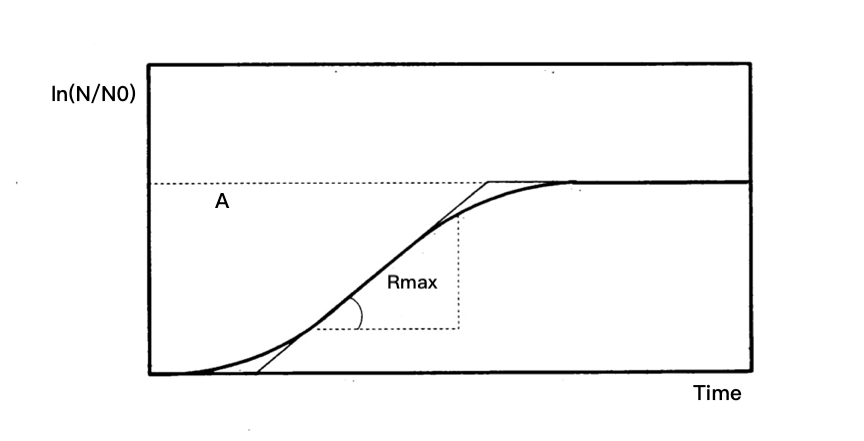
\includegraphics[width = \textwidth]{../results/images/fig4.png}
            \caption{$A$ growth curve}
            \label{fig4}
    \end{figure}
    
    $H_0$: In baranyi model, $h_0$ can be related to $t\textsubscript{lag}$ and $r\textsubscript{max}$, which made it easily to be calculated:
    
    \begin{equation}
	    t_{lag}= \frac{1+\frac{1}{h_0}}{r_{max}}
	\end{equation}
	So:
	\begin{equation}
	    h_0 = \frac{1}{e^{r_{max}t_{lag}}-1}
	\end{equation}
	
	$\mu$:  In Buchanan model, $\mu$ value is calculated by the equation below\citep{damert1994abacus}:
	\begin{equation}
	    \mu = \frac{N_{max}-N_0}{t_{max}-t_{lag}}
	\end{equation}
	After all the starting values are confirmed, I built new columns to store them in data frame
	
	\subsection{NLLS fitting}
	Here, I use the Python package LMFIT\citep{newville2016lmfit} for each model to apply model fitting on each curve by NLLS method. The main task for doing a non-linear least-squares fit of a model to data is to write an objective function that takes the values of the fitting variables and calculates either a scalar value to be minimized, typically in the least-squares sense. Also, the objective function should return the value to be minimized. So, what I need to do is calculating objective residual to be minimized from parameters. Parameter is the quantity to be optimized in all minimization problems, the parameters are given the starting value as their initial value when first try. Then, assign parameters randomly from the range of normal distribution with the initial value as the axis. It is hope that the LMFIT can find the best parameter values for each model within the maximum try times. The residual is calculated as (model – data) with the best give parameters.
	Note that the cubic model is a polynomial linear model and the best way to fit this model might be the Ployfit funtion in Numpy for Python, but in this study I still used LMFIT package because I want to test if this package designed for non-linear model fitting could also applied in linear model fitting. It turns out that LMFIT not only can fit the non-linear model, but also available in linear model. 
	
	\subsection{Model Selection}
	Many model selection methods are used to find the optimal model, like $R\textsuperscript{2}$, $AIC$, $BIC$. Here I choose the Akaike information criterion ($AIC$) as my main method. the $AIC$ value of the model is the following:
    \begin{equation}
        AIC = 2\rho+\ln (L)
    \end{equation}
    
    Where $\rho$ is the number of estimated parameters in the model; $L$ is the maximum value of the likelihood function for the model\citep{mcelreath2016statistical}. 
    
    When the sample size is small, there is a substantial probability that $AIC$ will select models that have too many parameters, i.e. that $AIC$ will over fit\citep{mcquarrie1998regression}. To address such potential over fitting, $AICc$ was developed: $AICc$ is $AIC$ with a correction for small sample sizes\citep{cavanaugh1997unifying}.
    
    \begin{equation}
        AICc = AIC + \frac{2\rho^{2}+2\rho}{n-\rho-1}
    \end{equation}
    
    Comparing to the other methods, the formula for the Bayesian information criterion ($BIC$) is similar to $AIC$, but with a different penalty for the number of parameters. With $AIC$ the penalty is $2\rho$, whereas with BIC the penalty is $\ln$(n)$\cdot$$\rho$.
    
    A comparison of $AIC$/$AICc$ and $BIC$ is given by Burnham and Anderson \citep{burnham2002model}, with follow-up remarks by Burnham and Anderson\citep{burnham2004multimodel}. The authors show that $AIC$/$AICc$ can be derived in the same Bayesian framework as $BIC$, just by using different prior probabilities. In $BIC$, though, each candidate model has a prior probability of $1$/$R$, where $R$ is the number of candidate models. Such a derivation is 'not sensible', because the prior should be a decreasing function of $\rho$. Additionally, the authors present a few simulation studies that suggest $AICc$ tends to have practical/performance advantages over BIC\citep{burnham2004multimodel}.
    
    As for $R\textsuperscript{2}$, although it is the simplest way to compare two models in terms of fitting(eq15). It calculated from Residual Sum of Squares ($RSS$) and Total Sum of Squares ($TSS$). However, it neglects the complexity of the model, which would lead to a situation that a very complicated model with lots of parameters has been chosen just because it converges best. In order to avoid this problem, $AIC$ provide a better choice because it considers about the complexity of models and penalises the over-fitting\citep{bozdogan1987model}. Equation of calculating $AIC$ contains the number of parameters in model(eq16). 
    
    \noindent\begin{minipage}{0.5\linewidth}
    \begin{equation}
        R^2 = 1 - \frac{\textrm{RSS}}{\textrm{TSS}}
	\end{equation}
    \end{minipage}%
	\begin{minipage}{0.5\linewidth}
	\begin{equation}
        AIC = N\ln{\frac{RSS}{N}} + 2\rho
	\end{equation}
	\end{minipage}\par\vspace{\belowdisplayskip}
	
	After getting the $AIC$ and $AICc$ for each curve, $\Delta$AIC and $\Delta$AICc would then be calculated as the difference between the lowest $AIC$($AICc$) and the $AIC$($AICc$) for each model. If $\Delta$AIC or $\Delta$AICc was less than or equal to 2, then the corresponding model can be regarded as the best model\citep{burnham2004multimodel}.
	
	The Akaike weight $W_i$(AIC) was then calculated for each model by below equation. This method can provide the likelihood of each model being the best choice, which promotes the interpretation of comparing models. $W_i$ (AICc) had also been calculated for analysis\citep{wagenmakers2004aic}.
	\begin{equation}
        W_i = \frac{\exp\{-\frac{1}{2}\Delta_i\}}{\sum_{j=1}^{R} \exp\{-\frac{1}{2}\Delta_j\}}
    \end{equation}
    
    \subsection{Computing languages}
    Python 3.5.2 was used for arranging data, estimating starting values of parameters in population growth models and model fitting with NLLS. Using library pandas to manipulate the large database easily. It is quickly to use Numpy and Scipy to get the estimate values\citep{mckinney2011pandas}. Choosing Python’s LMFIT package rather than R is because when facing the large database and complicated calculating process, Python often does better and faster than R.
    
    R version: 3.2.3. R was used in model selection stage by its’ calculating function because it is user-friendly. The drawing process also used R, because the ggplot2 library can produce very accurate and high quality figures\citep{ginestet2011ggplot2}.
    
    GNU bash, version 4.3.48(1). The Bash Shell was used to tie all the scripts in this project as a workflow and compile the report from latex script to pdf file.
    
\section{Results}
After manipulating original database, there are 295 curves. Among the five models, except the classical mechanistic model has several unfitted subsets, the success fitting rate of other models are 100\%. So, I plot the models in one data subset to observe the actual fitting imagine.

\begin{figure}[H]
    \centering
	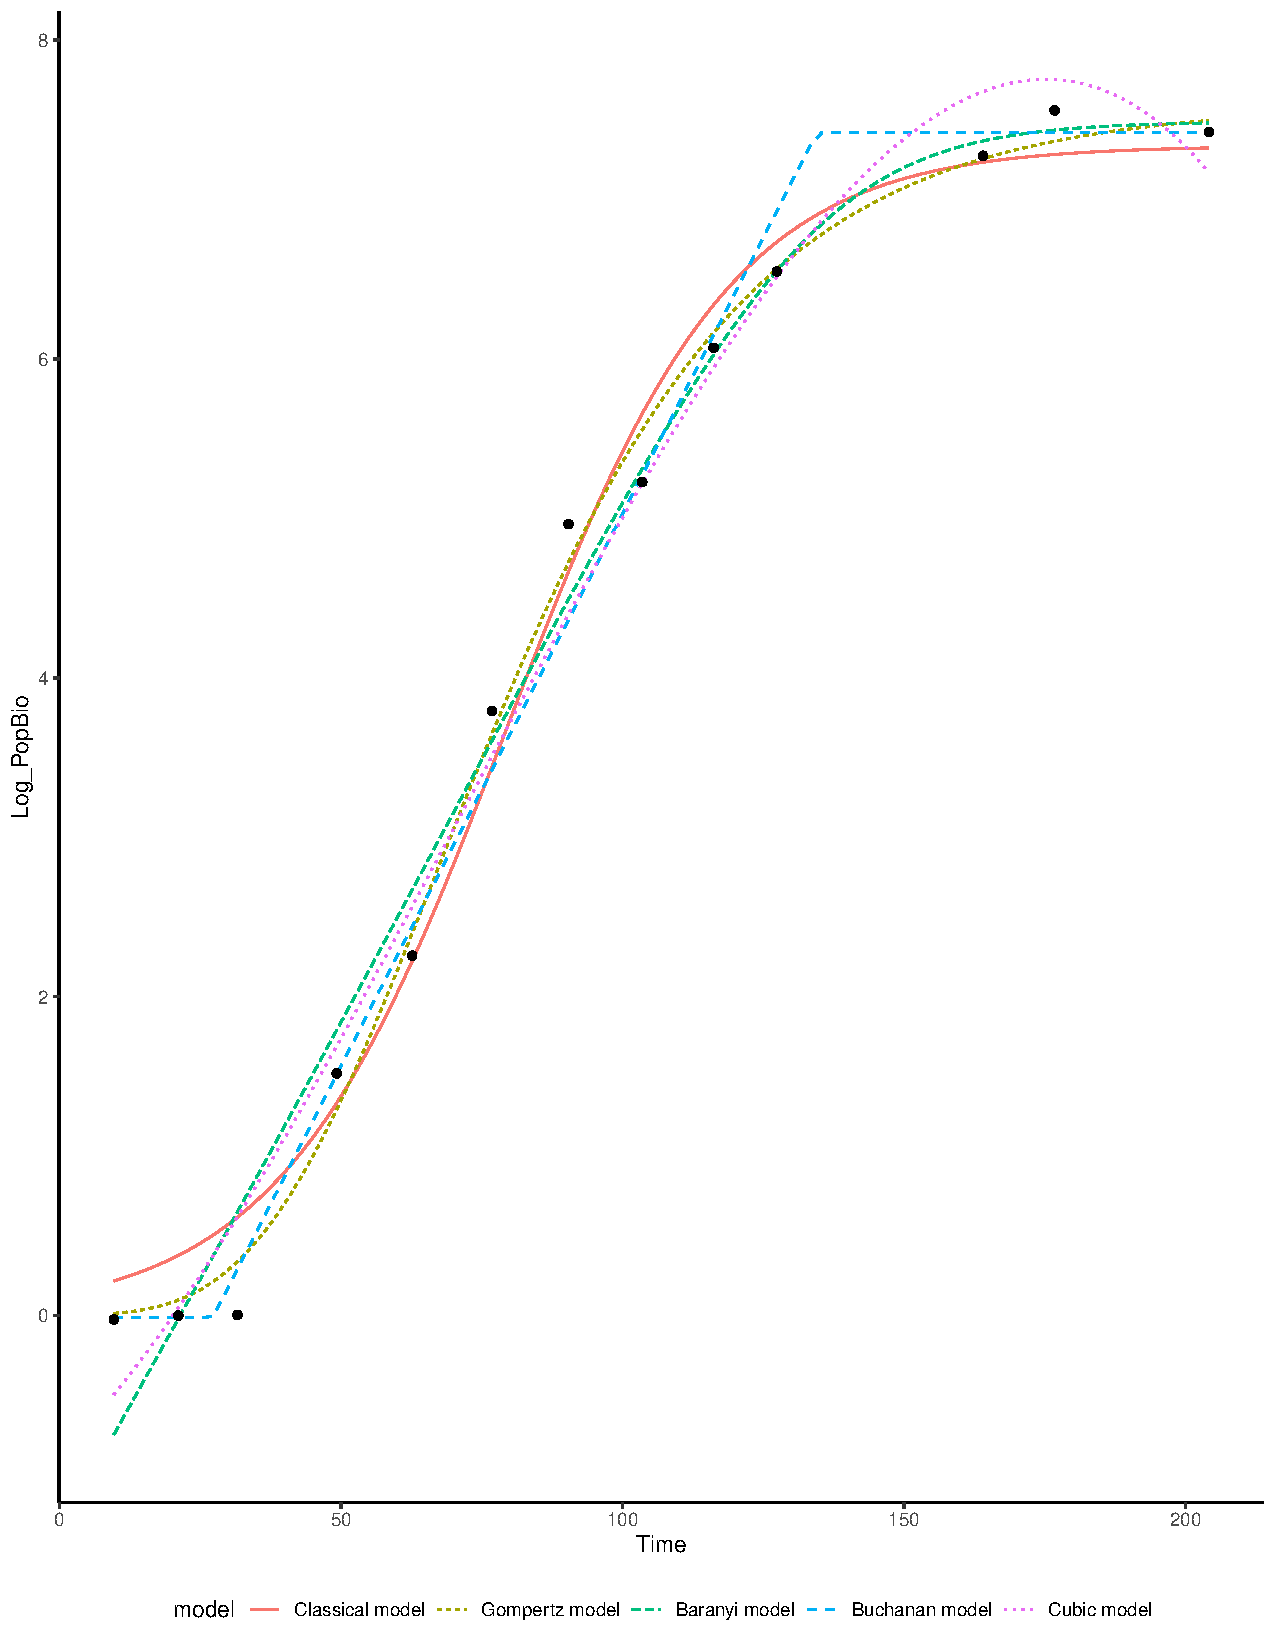
\includegraphics[width = \textwidth]{../results/images/135_plot.pdf}
    \caption{Comparison five models’ curves. X axis represents the time and Y axis represents logged population size of Pseudomonas. The data was taken from (Galarz, L.A., Fonseca, G.G. and Prentice, C., 2016) The analysis information for comparison between each model are listed in the table below.}
    \label{fig5}
\end{figure}

\begin{table}[H] \centering
    \resizebox{\textwidth}{!}{%
    \begin{tabular}{c|ccccccc}
        \hline
        Model & $R^2$ & $AIC$ & $AIC_c$ & $\Delta$$AIC$ & $\Delta$$AIC_c$ & Weight($AIC$) & Weight($AIC_c$) \\
        \hline
        Classical & $0.989$ & $-24.93$ & $-22.26$ & $13.32$ & $13.32$ & $0.0013$ & $0.0013$\\
        Gompertz & $0.996$ & $-38.25$ & $-35.58$ & $0$ & $0$ & $0.9922$ & $0.9983$\\
        Baranyi & $0.986$ & $-20.28$ & $-15.28$ & $17.97$ & $20.31$ & $0.0001$ & $3.88e - 5$\\
        Buchanan & $0.992$ & $-28.12$ & $-19.55$ & $10.13$ & $16.03$ & $0.0062$ & $0.0003$\\
        Cubic & $0.987$ & $-20.89$ & $-15.89$ & $17.36$ & $19.70$ & $0.0002$ & $5.28e - 5$\\
        \hline
    \end{tabular}}
    \caption{$R^2$, AIC, AICc, $\Delta$AIC, $\Delta$AICc and Akaike Weight for each model curve in fig2}
    \label{table2}
\end{table}

It seems that all the five models are fitted nicely in this data subset, so it’s hard to say which one is the best from the eyeballing way. However, from the details in table2, we can clearly find that the Gompertz model is the best fitted model for this data subset, because it has the minimum value of $AIC$, $AICc$, $\Delta$$AIC$ and $\Delta$$AIC_c$, also with the maximum value in Weight($AIC$) and Weight($AICc$).

Let's have an overall statistical analysis among the five models. Tables below show the  statistical analysis information in overall scale.

\begin{table}[H] \centering
    \begin{tabular}{c|c|c}
        \hline
        Model & $\Delta$AIC$\leqslant2$ & $\Delta$AICc$\leqslant2$ \\
        \hline
        Classical & 139 & 169\\
        Gompertz & 68 & 79\\
        Baranyi & 91 & 73\\
        Buchanan & 82 & 45\\
        Cubic & 133 & 65\\
        \hline
    \end{tabular}
    \caption{$\Delta$AIC and $\Delta$AICc in each model less than 2 will be counted across all curves} 
    \label{table3}
\end{table}

From table3, it is observed that Classical mechanistic model has the largest number of data subset with both $\Delta$$AIC$ and  $\Delta$$AICc$ less than 2, that means the Classical mechanistic model has the best fitting curve. Note that Cubic model also has a high proportion in the number of $\Delta$$AIC$ less than 2, but the number of $\Delta$$AICc$ less than 2 is decreased dramatically. So I made two box plotting to compare the $AICc$ values and Weight($AICc$) values of each model. 

\begin{figure}[H]
    \centering
	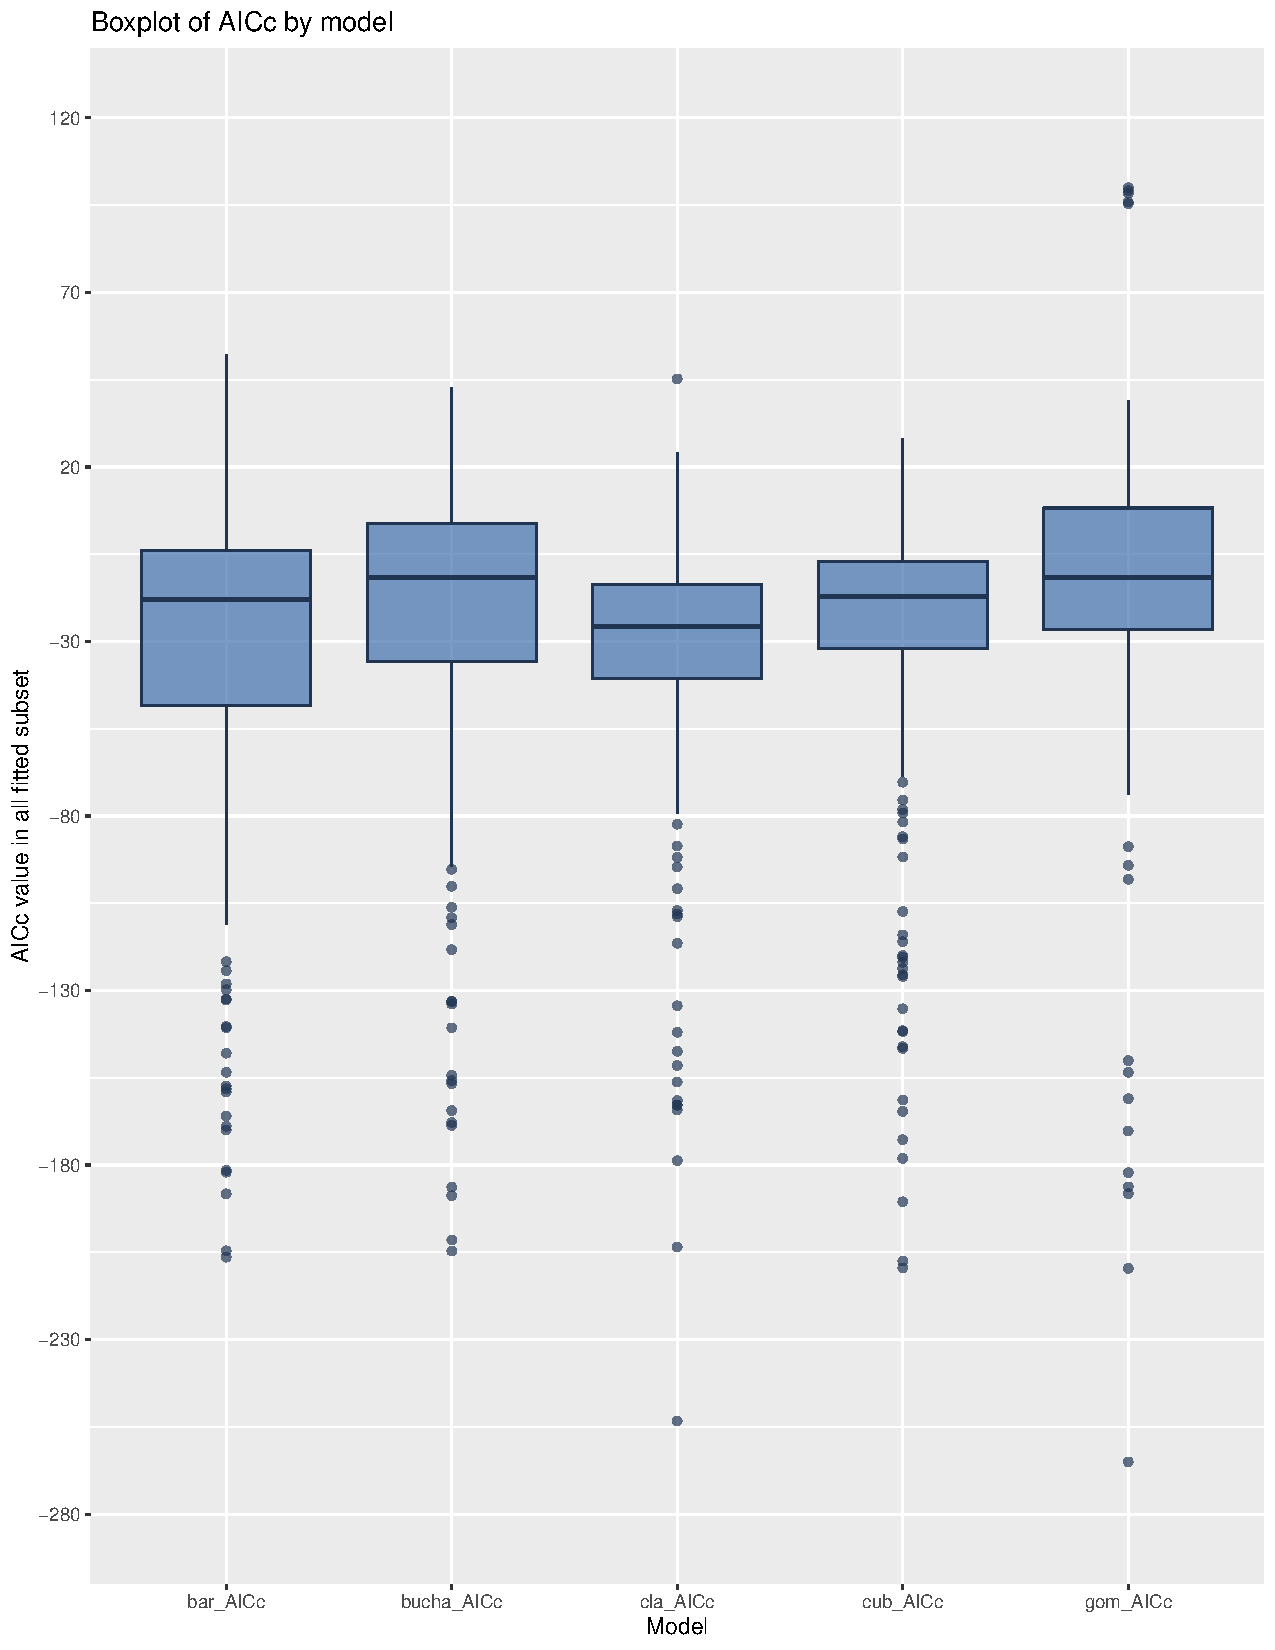
\includegraphics[width = \textwidth]{../results/images/boxplot.pdf}
    \caption{Box plot, shows the $AICc$ value distribution in each model}
    \label{fig6}
\end{figure}

\begin{figure}[H]
    \centering
	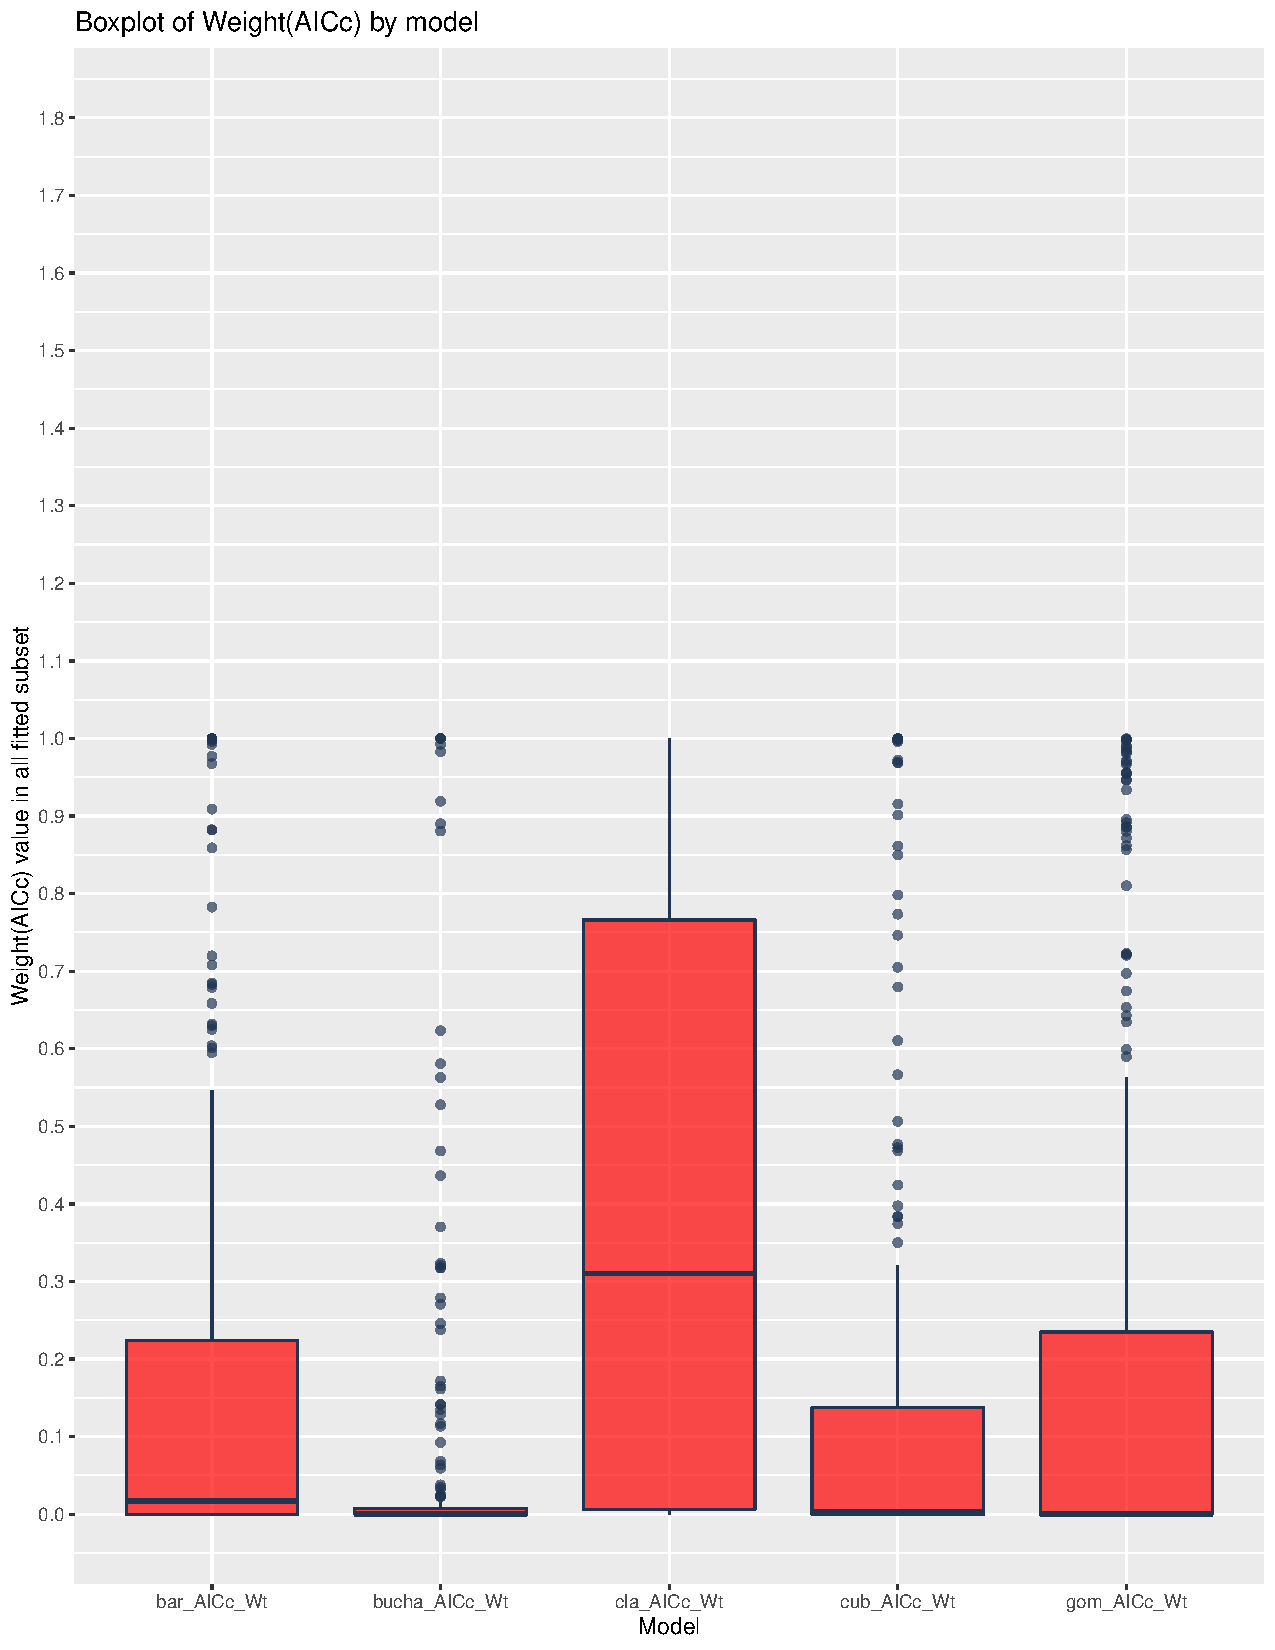
\includegraphics[width = \textwidth]{../results/images/boxplot_2.pdf}
    \caption{Box plot, shows the Akaike Weight (AICc) distribution in each model}
    \label{fig7}
\end{figure}

In Fig6, the classic mechanistic model has a slight advantage over other models in the average value of $AICc$. In Fig7, this advantage significantly increased in the Weight ($AICc$) scale. Thus proves that the classic mechanistic model is the best model for this database.
Also, there is a table shows all the mean statistic information of the models.

\begin{table}[H] \centering
    
    \resizebox{\textwidth}{!}{%
    \begin{tabular}{c|ccccc}
        \hline
        Model & Mean $R^2$ & Mean $AIC$ & Mean $AICc$ & Mean Akaike Weight($AIC$) & Mean Akaike Weight($AICc$)\\
        \hline
        Classical & 0.8681 & -31.9921 & -34.2791 & 0.2628 & 0.3926\\
        Gompertz & -1.0264 & -16.3720 & -15.1259 & 0.1343 & 0.1876\\
        Baranyi & 0.8332 & -30.7859 & -33.8439 & 0.1807 & 0.2038\\
        Buchanan & 0.8091 & -30.17447 & -24.9660 & 0.1769 & 0.0693\\
        Cubic & 0.8988 & -31.8501 & -30.4140 & 0.2452 &  0.1467\\
        \hline
    \end{tabular}}
    \caption{Mean values of $R^2$, AIC, AICc, Akaike Weight(AIC) and Akaike Weight(AICc) in each model.} 
    \label{table4}
\end{table}   

\section{Discussion}
Although the classical mechanistic model did not match $100\%$ of all subsets successfully, from the final statistics, it is still the best model to fit the bacteria growth curve under the given database. The support evidence is shown in table3, table4, the classical mechanistic model owns the minimum value of mean $AIC$ and mean $AICc$, the most times to be the best model ($\Delta$$AICc$ $\leq$ 2) and the biggest likelihood of being the best model (Akaike weight)\citep{sakamoto1986akaike}. As for the other models, they have shown good performance in the fitting process as well. Like Gompertz model, it used to be the best fit in some data subsets, however, it is not satisfactory in other data subsets. After my observation, I think the reason may be related to the size of the population in the data. In some subsets that use larger orders of magnitude as units, the population size becomes very small, which makes the values of $A$ and $t\textsubscript{lag}$ extremely small. In this situation, Gompertz model is easy to linearize and the outcome become not so well. cubic is a classic mathematical model, and it is also a universal model for many biological phenomena. Although the success rate of its model fitting is $100\%$, through the plotting of some subsets, it can be found that the fitting curve of cubic model is more inconsistent with the actual situation compared with other models. Because the cubic model does not have any biologically significance\citep{brunner2006matrix}, it is not recommended as a predictive model for estimating bacterial growth trends. What surprised me most is the buchanan model. As a three-segment linear model, I was not optimistic about it when I first saw it. I think the fitting result may be very poor because it looks too different from the growth curve. But the final fitting results are very nice, not only all the subsets are fitted successfully but also it has lower $AICc$ and higher fitting likelihood than some other models. The reason may belong to its biological similarity with the characteristics of the bacterial growth. Each of the three-line segments correspond to a bacterial growth period. The three-phase linear model seems to be the simplest, effective primary model that can be used readily with curve fitting software to estimate bacterial growth kinetics\citep{buchanan1997simple}.

\bibliographystyle{agsm}
\bibliography{writeup}
    
\end{document}
